% Options for packages loaded elsewhere
\PassOptionsToPackage{unicode}{hyperref}
\PassOptionsToPackage{hyphens}{url}
\PassOptionsToPackage{dvipsnames,svgnames,x11names}{xcolor}
%
\documentclass[
  12pt,
  oneside]{book}
\usepackage{amsmath,amssymb}
\usepackage{lmodern}
\usepackage{iftex}
\ifPDFTeX
  \usepackage[T1]{fontenc}
  \usepackage[utf8]{inputenc}
  \usepackage{textcomp} % provide euro and other symbols
\else % if luatex or xetex
  \usepackage{unicode-math}
  \defaultfontfeatures{Scale=MatchLowercase}
  \defaultfontfeatures[\rmfamily]{Ligatures=TeX,Scale=1}
\fi
% Use upquote if available, for straight quotes in verbatim environments
\IfFileExists{upquote.sty}{\usepackage{upquote}}{}
\IfFileExists{microtype.sty}{% use microtype if available
  \usepackage[]{microtype}
  \UseMicrotypeSet[protrusion]{basicmath} % disable protrusion for tt fonts
}{}
\makeatletter
\@ifundefined{KOMAClassName}{% if non-KOMA class
  \IfFileExists{parskip.sty}{%
    \usepackage{parskip}
  }{% else
    \setlength{\parindent}{0pt}
    \setlength{\parskip}{6pt plus 2pt minus 1pt}}
}{% if KOMA class
  \KOMAoptions{parskip=half}}
\makeatother
\usepackage{xcolor}
\IfFileExists{xurl.sty}{\usepackage{xurl}}{} % add URL line breaks if available
\IfFileExists{bookmark.sty}{\usepackage{bookmark}}{\usepackage{hyperref}}
\hypersetup{
  colorlinks=true,
  linkcolor={MidnightBlue},
  filecolor={Maroon},
  citecolor={Blue},
  urlcolor={Blue},
  pdfcreator={LaTeX via pandoc}}
\urlstyle{same} % disable monospaced font for URLs
\usepackage[left=3cm,top=2.5cm,right=3cm,bottom=2.5cm]{geometry}
\usepackage{longtable,booktabs,array}
\usepackage{calc} % for calculating minipage widths
% Correct order of tables after \paragraph or \subparagraph
\usepackage{etoolbox}
\makeatletter
\patchcmd\longtable{\par}{\if@noskipsec\mbox{}\fi\par}{}{}
\makeatother
% Allow footnotes in longtable head/foot
\IfFileExists{footnotehyper.sty}{\usepackage{footnotehyper}}{\usepackage{footnote}}
\makesavenoteenv{longtable}
\usepackage{graphicx}
\makeatletter
\def\maxwidth{\ifdim\Gin@nat@width>\linewidth\linewidth\else\Gin@nat@width\fi}
\def\maxheight{\ifdim\Gin@nat@height>\textheight\textheight\else\Gin@nat@height\fi}
\makeatother
% Scale images if necessary, so that they will not overflow the page
% margins by default, and it is still possible to overwrite the defaults
% using explicit options in \includegraphics[width, height, ...]{}
\setkeys{Gin}{width=\maxwidth,height=\maxheight,keepaspectratio}
% Set default figure placement to htbp
\makeatletter
\def\fps@figure{htbp}
\makeatother
\setlength{\emergencystretch}{3em} % prevent overfull lines
\providecommand{\tightlist}{%
  \setlength{\itemsep}{0pt}\setlength{\parskip}{0pt}}
\setcounter{secnumdepth}{5}
%----------------------------------------------------
% 	CONFIGURATION OF PARAMETERS
%----------------------------------------------------

% ----------------
%  FONTS AND TYPESETTING SETTINGS
% -----------------
\usepackage[french]{babel}
%\usepackage[bitstream-charter]{mathdesign}

\usepackage{fontawesome5}
\usepackage{academicons}
\usepackage[notransparent]{svg}
\usepackage{tabu}
%\usepackage{coloremoji}
%\usepackage{emoji}

\usepackage{longtable}

%\usepackage[tracking=smallcaps]{microtype}
%\usepackage[bitstream-charter]{mathdesign}

% ----------------
%  STYLES OF THE CHAPTER, SECTION
% -----------------
%Options: Sonny, Lenny, Glenn, Conny, Rejne, Bjarne, Bjornstrup
\usepackage[Bjornstrup]{fncychap}
\usepackage{marginnote}
\renewcommand*{\marginfont}{\small\sffamily}

%---------------------------------
% Modification du model de UL
%\graphicspath{{./Figures/}} % chemin des figures


% -----------------
%  DEFINITION OF THE COLORS
% -----------------
%\usepackage{color} % Color
%\usepackage[usenames,dvipsnames,table]{xcolor}
%\usepackage{colortbl}

% -----------------
% 	MATHEMATHICAL SYMBOLS
% -----------------
%\usepackage{amssymb} %% The amssymb package provides various useful mathematical symbols
%\usepackage{amsthm} %% The amsthm package provides extended theorem environments
%\usepackage{amsmath}  % Paqute de Matematicas
%----------------------------------------------------------------------------------------

% -----------------
%  BIBLIOGRAPHY
% -----------------
%\usepackage  {natbib}
\usepackage{csquotes} %a utiliser si biblatex est utilisé
%\usepackage[style=numeric-comp, doi=false, backend=bibtex, isbn=false, url=false, sorting=none, language=english ]{biblatex}
%\addbibresource{library.bib}


\usepackage{booktabs}
% -----------------
%  VARIOUS PACKAGES FROM ME
% -----------------
%\usepackage{minitoc}
%\usepackage{booktabs} % Horizontal rules in tables
%\usepackage{float} % Required for tables and figures in the multi-column environment - they need to be placed in specific locations with the [H] (e.g. \begin{table}[H])
%\usepackage[lofdepth,lotdepth]{subfig} 
%\usepackage{multirow} % Use multirows in the tables

%\usepackage {textcomp} % (Symbols Euros)
%\usepackage{nomencl} % nomenclature package
%\usepackage{soul}
%\renewcommand\thesection{\arabic{section}} %Redefinition of numeration of the document
%\usepackage{pdflscape} % hacer el documento lanscape en las hojas
%\usepackage{enumitem} % offers ready-made options for eliminating the space between items and paragraphs within the list (noitemsep) or all vertical spacing (nosep): 

%\usepackage{afterpage} % For make blank pages
\usepackage{pdfpages} % For insert the title page.




% -----------------
%  VARIOUS PACKAGES FROM UNIVERSITE DE LORRAINE
% -----------------
%\usepackage{import}


%----------------------------------------------------------------------
%  PERSONALIZATION OF PACKAGES
%----------------------------------------------------------------------


% -----------------
%  DEFINITION OF COMMANDS BY ME
% -----------------
%\pagenumbering{Roman}


\usepackage{booktabs}
\usepackage{longtable}
\usepackage{array}
\usepackage{multirow}
\usepackage{wrapfig}
\usepackage{float}
\usepackage{colortbl}
\usepackage{pdflscape}
\usepackage{tabu}
\usepackage{threeparttable}
\usepackage{threeparttablex}
\usepackage[normalem]{ulem}
\usepackage{makecell}
\usepackage{xcolor}
\ifLuaTeX
  \usepackage{selnolig}  % disable illegal ligatures
\fi

\author{}
\date{\vspace{-2.5em}}

\begin{document}

\begin{titlepage}
	\begin{flushright}

		\LARGE{\textbf{2022}}\\
		\vfill
		\Large{Dossier de Candidature} \\ 
		\Large{aux} \\
		\Large{fonctions de Maître de conférences}\\[1cm]
		\Large{\textbf{Référence 60-62MCF 0182 -- Galaxie 1473}}  \\
		\vfill
		
      \Large{École Nationale Supérieure en Génie des Systèmes Industriels --ENSGSI-}\\
      \Large{Équipe de Recherche sur les Processus Innovatifs --ERPI-}\\
      \vfill
		\Large{\textbf{Dossier adressé aux rapporteurs}}\\
		\vfill
	%	\large Presente par\\
		\Large \textbf{Fabio Alberto CRUZ SANCHEZ}\\[1cm]
		\normalsize Qualification aux fonctions de maître de conférences \\
		No  campagne 2019 60ème  section CNU \\
		No  campagne 2019 62ème  section CNU \\
%		Laboratoire ERPI -- Équipe de Recherche sur les Processus Innovatifs\\
%		8 rue Bastien Lepage - BP 90647\\ 
%		54010 NANCY cedex\\ 
		E-mail: \href{cruzsanc1@univ-lorraine.fr}{cruzsanc1@univ-lorraine.fr}  \\ 
		Tel: +33 7 78 78 38 07  \\ 
		\vfill
		\hrule 
		\vspace{5pt}
		\begin{center}
			\Large{\textbf{S\hspace{7pt}E\hspace{7pt}C\hspace{7pt}T\hspace{7pt}I\hspace{7pt}O\hspace{7pt}N \hspace{25pt}   C\hspace{7pt}N\hspace{7pt}U \hspace{25pt}   6\hspace{7pt}0 / 6\hspace{7pt}2 } }\\
		\end{center}
		\vspace{5pt} 
		\hrule
		%\vfill
		\vspace{25pt} 
		
		%\includegraphics[width=0.3\linewidth]{Figures/CNU-logo.png}\\ 
		
		
	\end{flushright}
\end{titlepage}

{
\hypersetup{linkcolor=}
\setcounter{tocdepth}{1}
\tableofcontents
}
\hypertarget{curriculum-vitae}{%
\chapter{Curriculum Vitae}\label{curriculum-vitae}}

\begin{minipage}{0.35\linewidth}

\begin{center}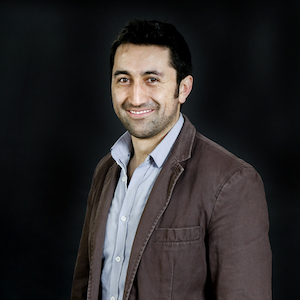
\includegraphics[width=0.6\linewidth]{/Users/fabio/Documents/4-Projects/MdC/Poste-ENSGSI/Figures/Fabio} \end{center}
\end{minipage}
\begin{minipage}{0.60\linewidth}

Franco-Colombien, Né le 06/05/1988 à Bogota, Colombie  \\
27, Rue du Pont de Pierre, 54270 - Essey-les-Nancy \\
Tel : 07.78.78.38.07 \\


\faEnvelope[regular] \href{mailto:fabbiocrux.ms@gmail.com}{fabbiocrux.ms@gmail.com} \\
\faGithub~\href{https://github.com/fabbiocrux}{Open Science with Github} \\

\includegraphics[width=1.5ex]{Figures/icons/google-scholar-square.pdf}  \href{https://scholar.google.fr/citations?user=8Cuoaf4AAAAJ&hl=fr}{Google scholar} \\


Recyclagé distribué; 3D Printing; Recyclage plastique; Soutenabilité
 
\end{minipage}

\hypertarget{pruxe9sentation}{%
\section{Présentation}\label{pruxe9sentation}}

Je suis ingénieur mécanique formé à l'Université Nacional de Colombie, titulaire d'un Master II en Management de l'Innovation et du Design Industriel et PhD. en Génie des Systèmes Industriels de l'Université de Lorraine. Mes expériences professionnelles et de recherche sont centrées sur le champ de la fabrication additive open source (également appelé \emph{Impression 3D}) comme vecteur de développement industriel durable.

Mon parcours est fortement lié à la recherche et au développement d'une nouvelle filière distribuée en circuit court pour la valorisation des matières plastiques recyclées via la fabrication additive. Cela implique une approche multi-échelle afin d'appréhender les enjeux liés au procédé technologique, la filière associée et le contexte territorial tout en gardant une collaboration avec de multiples acteurs et la mobilisation de différentes méthodologies pour améliorer, tester et expérimenter de nouveaux usages.

Je travaille sur un premier axe portant sur la validation du procédé d'impression 3D open source en tant qu'outil reproductible pour la fabrication des pièces en lien avec le Laboratoire LEM3 de l'UL. Une attention particulière est portée sur la performance géométrique, mécanique et vibratoire de ce procédé à l'échelle industrielle standard.
Un deuxième axe central dans mon parcours est la faisabilité technique du recyclage des thermoplastiques pour les processus d'impression 3D. J'ai eu l'opportunité de travailler pendant ma thèse sur les caractérisations mécanique et chimique de la matière recyclée dans la chaîne d'impression en co-tutelle avec le Équipe de Recherche sur les Processus Innovatifs (ERPI) et le Laboratoire des Réactions et Génie des Procédés (LRGP --- UMR 7274) à Nancy.
Je collabore avec le groupe de recherche FAST (Free Appropriate Sustainability Technology) de Western University de Canada sur le développement open source hardware afin de continuer à démocratiser la technologie associé au recyclage distribué.
Une troisième axe en cours de développement est l'analyse de la soutenabilité de cette filière en collaboration avec l'équipe InSyTe de l'Université Technologique de Troyes.
Le développement d'indicateurs au-déla des technico-économiques intégrant la capacité de charge des écosystèmes et leurs services est un enjeu prometteur pour rendre les filières industrielles plus résilientes.

Actuellement, je participe au développement du démonstrateur Green Fablab dans le cadre du projet Européen H2020 INEDIT.
Cela est une opportunité pour mieux comprendre l'opérationnalisation et la démultiplication de la démarche de recyclage distribué auprès des acteurs et des communautés locales.
En parallèle, je collabore également dans le projet Erasmus+ ClimateLabs que cherche à renforcer les capacités de recherche appliquée et d'innovation de dix universités partenaires du Mexique, du Brésil et de la Colombie par la conception et la mise en œuvre de Social Innovation Labs pour l'atténuation et l'adaptation au changement climatique.

\begin{figure}

{\centering 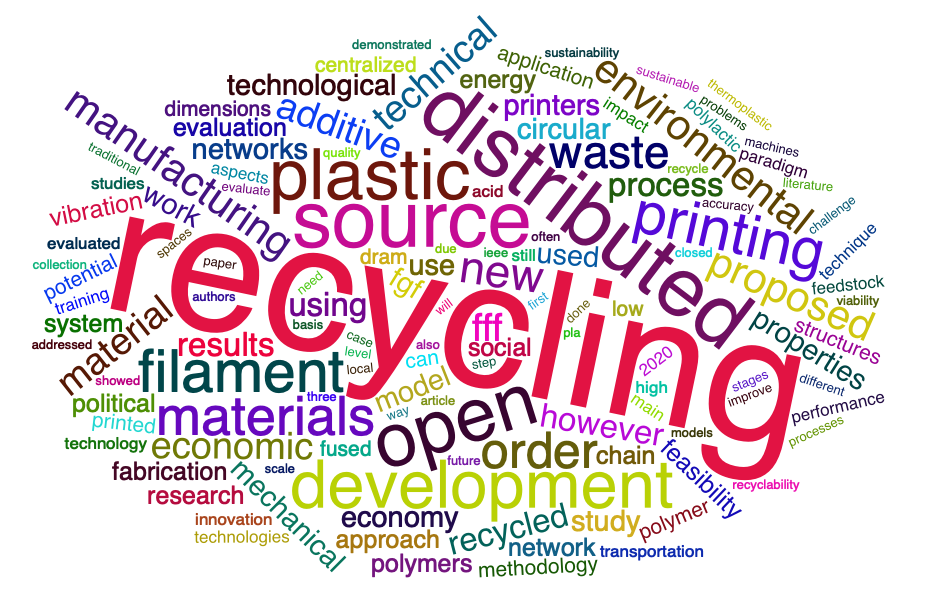
\includegraphics[width=0.8\linewidth]{/Users/fabio/Documents/4-Projects/MdC/Poste-ENSGSI/Figures/Cloud} 

}

\caption{Nuages de mots fait à partir des résumés des mes articles scientifique}\label{fig:unnamed-chunk-2}
\end{figure}

\hypertarget{formations}{%
\section{Formations}\label{formations}}

\begin{tabu} to \linewidth {X[0.4,l] X[2,l]}

2013 -- 2016 & \textbf{Ph.D., Université de Lorraine}, spécialité Génie des systèmes industriels \par
    Titre de thèse: \textbf{\emph{Methodological proposition to evaluate polymer recycling in open-source additive manufacturing contexts}} \par\vspace{5pt}
    
Défendu publiquement le 9 Décembre de 2016 à Nancy devant le jury:\par\vspace{5pt}

    \textbf{Rapporteurs:}
    \begin{itemize}
    
        \item \textit{Prof.} Nicolas PERRY --  ENSAM, Bordeaux - France
        \item \textit{Dr.} Salim BELOUETTAR -- LIST, Esch-sur-Alzette - Luxembourg
    \end{itemize}

\vspace{5pt}
    \textbf{Examinateurs:}
    \begin{itemize}
    
        \item \textit{Prof.} Joshua M. PEARCE -- MTU, Michigan - USA
        \item \textit{Prof.} Nadia BAHLOULI -- Université de Strasbourg, Strasbourg - France
        \item \textit{Prof.} Mauricio CAMARGO (\textit{Directeur}) -- UL, ERPI, Nancy - France
        
        \item \textit{MdC.} Hakim BOUDAOUD (\textit{co-directeur}) -- UL ERPI, Nancy - France
        
        \item \textit{Dr.} Sandrine HOPPE (\textit{co-directeur})  --  LRGP, Nancy - France
    \end{itemize}
        \\ [5pt]

2012 -- 2013 &
    \textbf{Master II.~ Management de l'Innovation et du Desing Industriel, Université de Lorraine, FR} \par Titre: \emph{Proposition d'un Protocole d'expérimentation standard pour la fabrication additive open source} \\[5pt]

2004 -- 2012 &
    \textbf{B.Sc. Ingénieur Mécanique}, Universidad Nacional de Colombia, Bogotá, Colombie \\
    
\end{tabu}

\hypertarget{expuxe9riences-professionnelles}{%
\section{Expériences Professionnelles}\label{expuxe9riences-professionnelles}}

\extrarowsep=3pt
\begin{tabu} to \linewidth {X[0.4,l] X[2,l]}
2022 -- ... &
    \textbf{Chercheur contractuel} Université de Lorraine, Université de Lorrain, Nancy -- France \\[5pt]

2021 -- 2021 &
    \textbf{Chercheur contractuel} Université de Technologique de Troyes, Équipe InSyTe (Anciennement CREIDD) Troyes -- France \\[5pt]

2017 -- 2021 &
    \textbf{Post-doctorant} Université de Lorraine, Université de Lorrain, Nancy -- France \\[5pt]

2010 -- 2011 & \textbf{International trainee} \href{http://www.mipengenharia.com.br/}{Entreprise MIP Engenharia S/A} \thinspace Belo Horizonte, Brazil \par
\textit{Projet:} Aide à la création d'un plan stratégique pour le projet d'internationalisation de MIP. Développement d'un benchmarking d'entreprises ayant un profil commercial similaire sur les marchés chilien, colombien et péruvien. \\
    
2008 -- 2009 &
    \textbf{Étudiant adjoint ingénieur} \emph{Universidad Nacional de Colombia. Bogotá - Colombia}  \par 
    \emph{Projet:} Conception et construction d'une machine de coulée centrifuge pour la fabrication de cylindres en fonte ASTM 40. \\
\end{tabu}

\hypertarget{compuxe9tences}{%
\section{Compétences}\label{compuxe9tences}}

\extrarowsep=3pt
\begin{tabu} to \linewidth {X[0.1,l] X[2,l]}

\faIcon{language}  & 

\includegraphics[width=2ex]{Figures/icons/flag-colombia.png} Langue Maternelle\quad 

\includegraphics[width=2ex]{Figures/icons/flag-france.png} Courante  \quad
\includegraphics[width=2ex]{Figures/icons/flag-usa.png} Courante  \quad
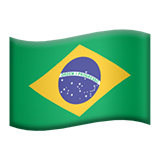
\includegraphics[width=2ex]{Figures/icons/flag-brazil.png} Professionnel \\[5pt] 


\faIcon{laptop}  & CAO (Solid-Works, Onshape), Matlab,  Data analysis / visualization, R, \textsc{Html, css} \\[5pt]
    

\faIcon{book}  & Academic research,  Mendeley, \LaTeX ~and Rmarkdown publishing.

\end{tabu}

\hypertarget{activituxe9s-de-recherche}{%
\chapter{Activités de Recherche}\label{activituxe9s-de-recherche}}

\hypertarget{synthuxe8se}{%
\section{Synthèse}\label{synthuxe8se}}

Dans la période 2014-2022, 7 articles dans des revues à comité de lecture et 5 conférences internationales ont été publiés comme illustré dans la Figure \ref{fig:bilan}.

Cette production scientifique relève des mes travaux de recherche mais aussi dans la participation des différents projets que j'ai eu l'opportunité de collaborer au sein du laboratoire ERPI.
Au courant de l'année 2022, 4 propositions d'articles ont été soumis à considération dans des revues à comité de lecture (en attente de décision) et 2 chapitres d'ouvrages collectifs orientés vers la communauté de recyclage de matériaux sont en cours de lecture par les éditeurs.

Le tableau montre les différents journaux auxquels nos propositions ont été publiées.
L'annexe \ref{articles} présente une liste complète de la production scientifique.

\begin{figure}

{\centering 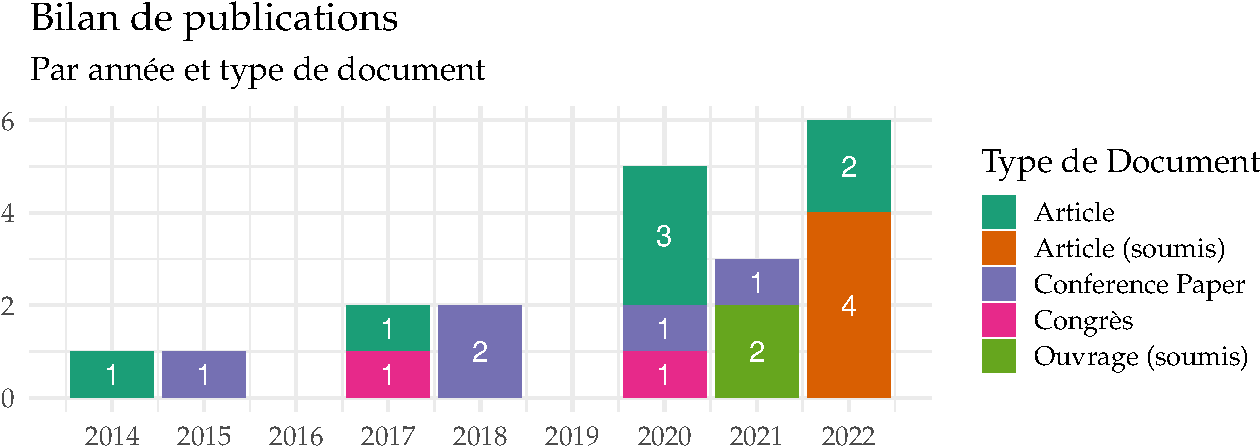
\includegraphics[width=0.8\linewidth]{Figures/bilan-1} 

}

\caption{Bilan de production scientifique}\label{fig:bilan}
\end{figure}

\begin{small}
\begin{minipage}{0.5\linewidth}

\begin{tabu} to \linewidth {X[2,l] X[0.5,l]}
\toprule
\textbf{Journals} & \textbf{IF (2020)} \\
\midrule
\href{https://www.journals.elsevier.com/additive-manufacturing}{Additive Manufacturing} & 10.998 \\
\href{https://www.journals.elsevier.com/resources-conservation-and-recycling}{Resources, Conservation \& Recycling} & 10.204\\

\href{https://www.journals.elsevier.com/journal-of-cleaner-production}{Journal of Cleaner Production} &  9.297\\
\href{https://www.tandfonline.com/toc/nvpp20/current}{Virtual and Physical Prototyping}
 & 8.092\\

\href{https://home.liebertpub.com/publications/3d-printing-and-additive-manufacturing/621/overview}{3D Printing and Additive Manufacturing}
 & 5.449\\
 
\href{https://www.springer.com/journal/11837}{JOM} & 2.474 \\
\href{https://www.journals.elsevier.com/cleaner-engineering-and-technology}{Cleaner Engineering and Technology} & -- \\


\bottomrule
\end{tabu}
\end{minipage}
\quad
\begin{minipage}{0.50\linewidth}
\begin{tabu} to \linewidth {X[0.2,c] X[2.5,l]}
\toprule
 & \textbf{Conferences et congrès} \\
\midrule
3 & Communications dans des conférences internationales en ingénierie et management de la technologie (ICE/IEEE) \\
2  & Communiations conferences sur la fabrication additive (Solid
Freeform Fabrication Symposium)  \\
1 & Participation aux congrès de la Société française de génie des procédés (SFGP) \\
1 & Participation à summer school (*spring of innovation and circular economy*) \\
\bottomrule
\end{tabu}
\end{minipage}
\end{small}

Mes activités de recherche ont comme dénominateur commun le croisement de trois enjeux sociétaux forts : 1) le vecteur industriel de la fabrication additive, 2) Celui du recyclage des matières plastique, 3) la croissance des espaces d'innovation dites ouverte type Fab Labs / hackerspaces. Chaque élément est très important dans un contexte où notre société doit agir à tous les niveaux (produit-procédé / filière / territoire) vers une transition écologique des modes de production, de fabrication et de consommation en prenant en compte les enjeux environnementaux actuels.

Mes travaux de recherche ont abouti à la proposition d'un cadre conceptuel de filière de recyclage des thermoplastiques pour l'impression 3D en considérant les étapes clés et un premier ensemble des indicateurs multicritères pour évaluer cette proposition comme illustré dans la figure Figure \ref{fig:DRAM}.

\begin{figure}

{\centering 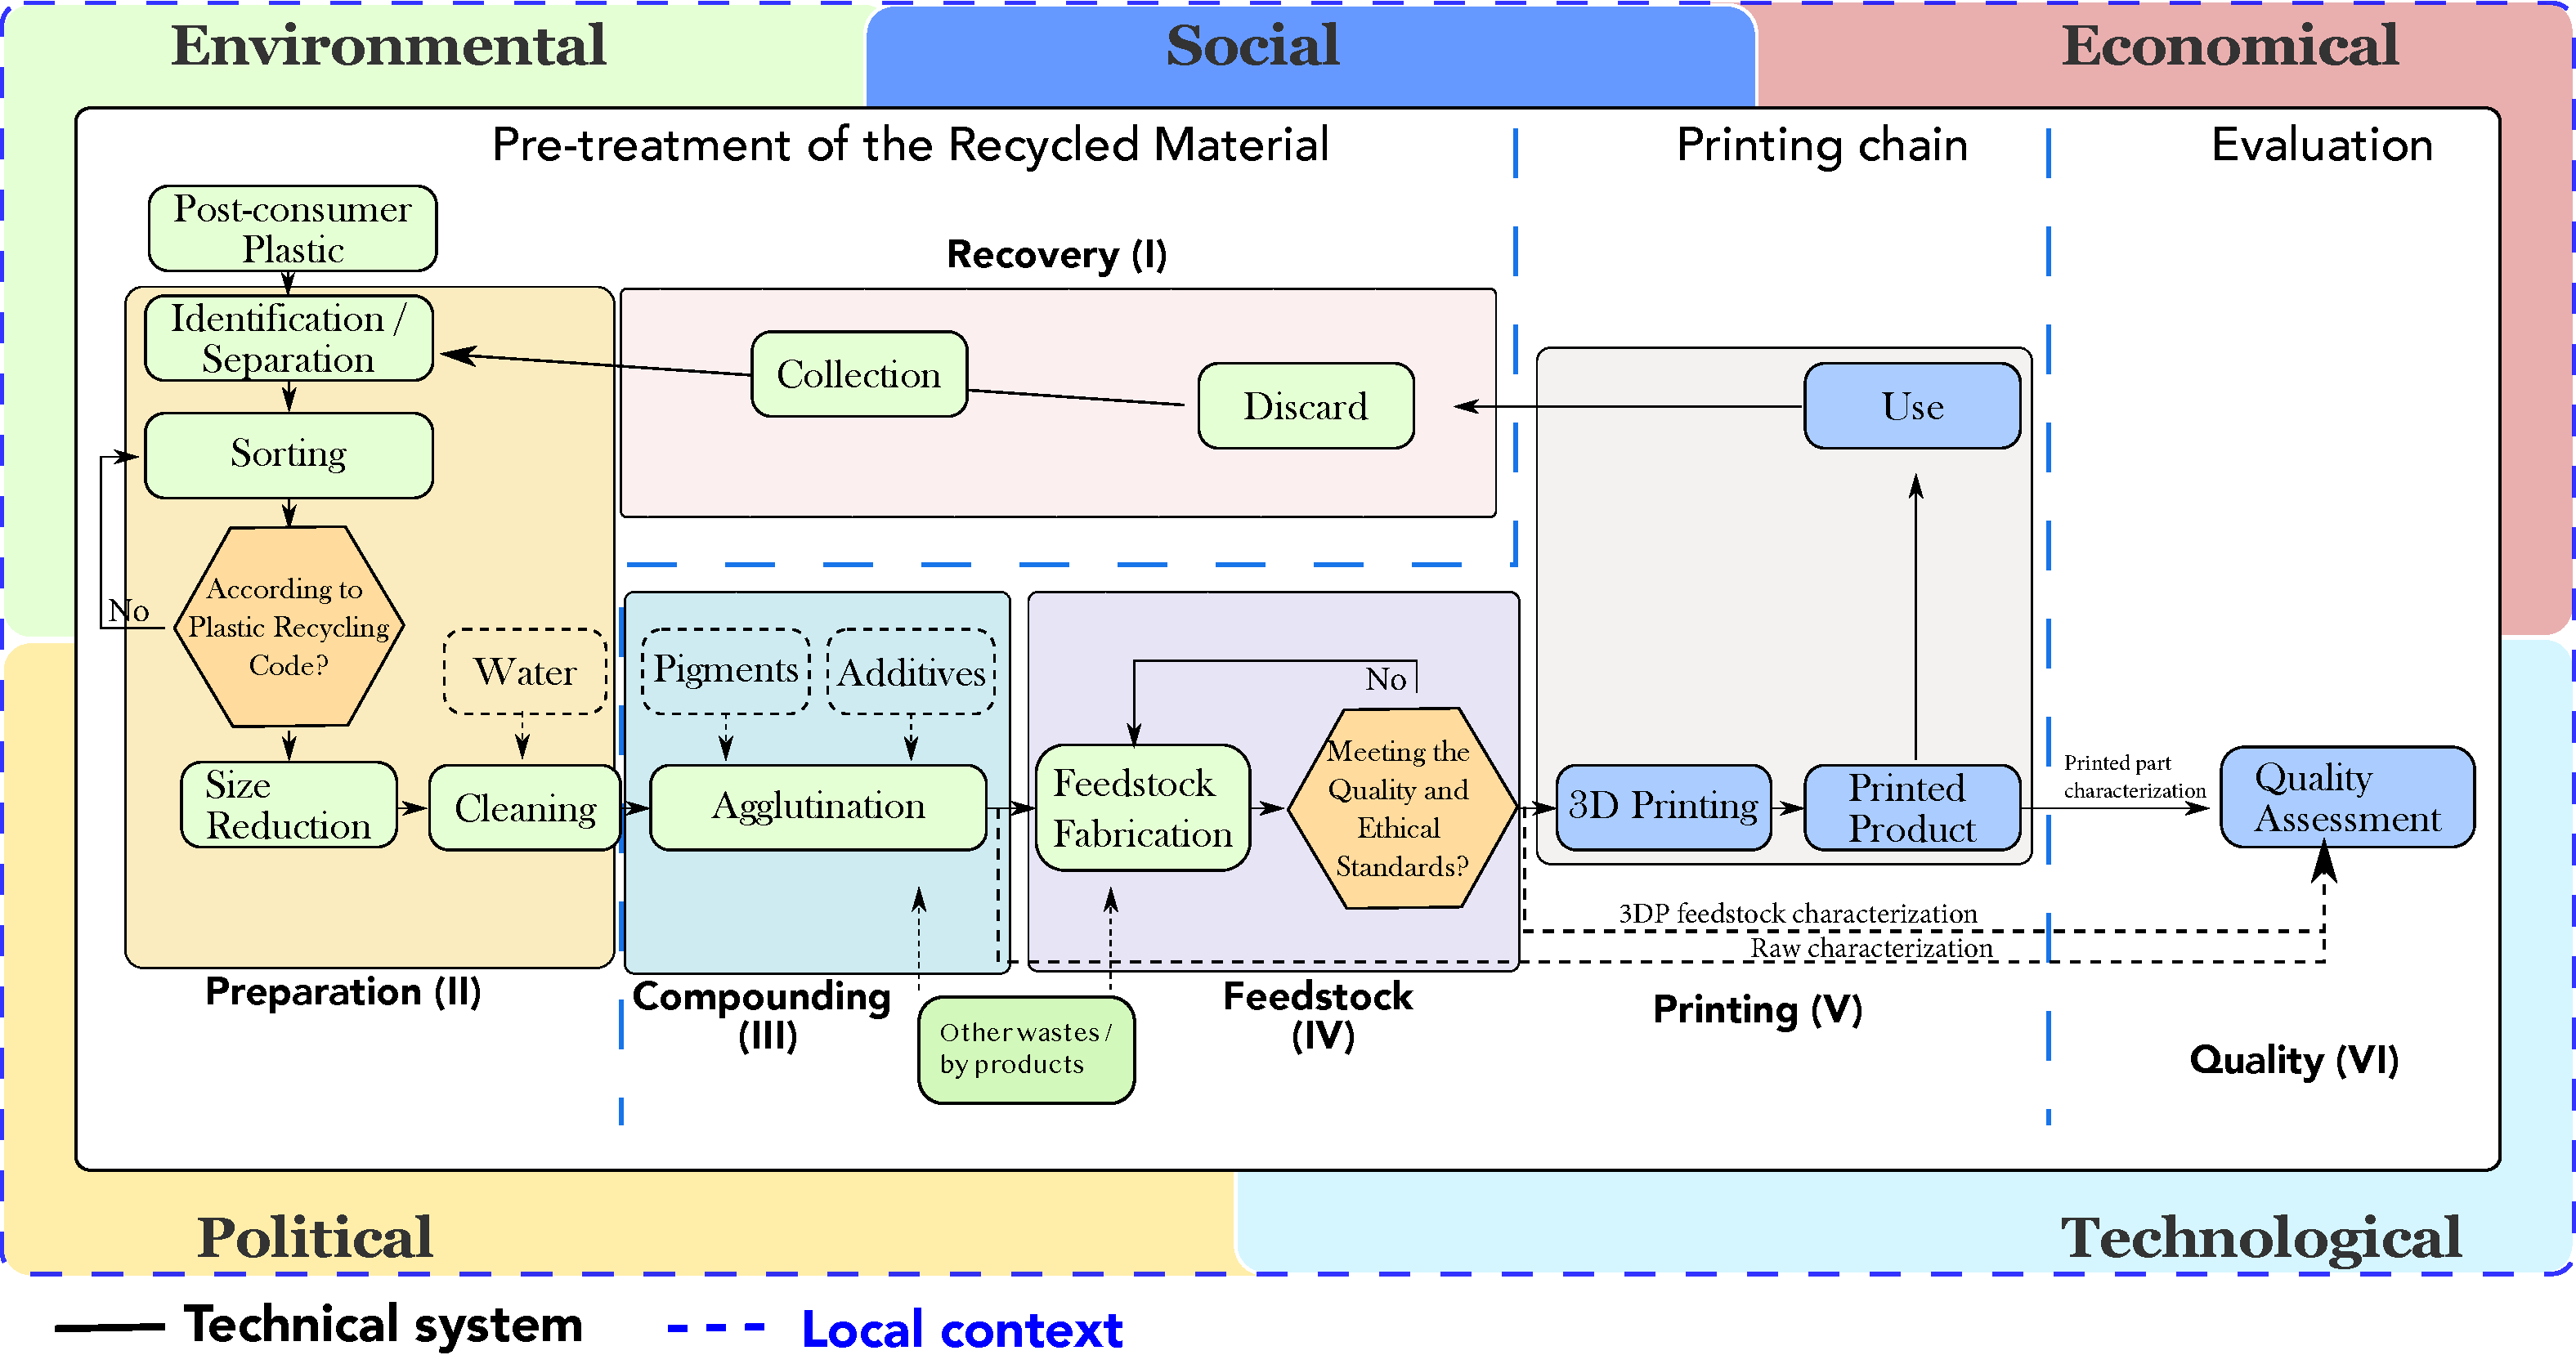
\includegraphics[width=0.9\linewidth]{/Users/fabio/Documents/4-Projects/MdC/Poste-ENSGSI/Figures/SDRAM-00} 

}

\caption{Récyclage distribué via la fabrication additive}\label{fig:DRAM}
\end{figure}

Je travaille avec différents collègues en France et à l'étranger pour pouvoir clarifier étape par étape les implications et les verrous scientifiques et technologiques afin de démocratiser une démarche locale de recyclage distribuée.

La particularité de la recherche que je développe au sein du laboratoire ERPI et dans la plateforme de recherche du Lorraine Fab Living Lab avec d'autres partenaires industriels et académiques est de pouvoir mieux comprendre autant la partie opérationnelle du système, mais également, l'implication systémique de cette nouvelle filière pour un territoire.

Aujourd'hui, dans le cadre du projet INEDIT, qui vise le transfert des approches `Do-It-Yourself' vers un context industriel, nous sommes en train de mettre en place un démonstrateur qui permettra tester l'approche appelé `Do-It-Together' dont la particularité est la connection de la co-création et la fabrication grâce à des plateformes numériques en incluant la réalité virtuelle (Figure \ref{fig:DRAM-INEDIT}).

\begin{figure}

{\centering 
\includegraphics[width=1\linewidth]{/Users/fabio/Documents/4-Projects/MdC/Poste-ENSGSI/Figures/INEDIT} 

}

\caption{Récyclage distribué via la fabrication additive}\label{fig:DRAM-INEDIT}
\end{figure}

Indéniablement, le développement de ce projet mobilise un panel de méthodologies de recherche dans la conception mécanique (e.g; plan d'expériences, validation statistique/ANOVA, simulation) et en innovation (e.g.~recherche opérationnelle, analyse multicritère, systèmes dynamiques) et ouvrent un champ d'expérimentation non négligeable pour la créativité de solutions avec des étudiants en ingénierie.

A partir de ce contexte, les axes de recherche peuvent être décrits d'un point de vue technologique (micro) vers une vision système (macro) de l'implication de la filière de recyclage en tant que système socio-technique.

\hypertarget{axes-de-recherche}{%
\section{Axes de Recherche}\label{axes-de-recherche}}

\hypertarget{limpression-3d-open-source-validation-des-standards-de-fabrication}{%
\subsection{L'impression 3D open source: validation des standards de fabrication}\label{limpression-3d-open-source-validation-des-standards-de-fabrication}}

La fabrication additive est reconnue comme un sujet avec une forte capacité disruptive qui est en train de changer les repères technologiques dans le domaine industriel, de conception \& design, et dans la société à une échelle globale.
Le principe de fabrication \emph{couche-par-couche} fait que ces procédés de fabrication offrent un espace à la conception mécanique et de manufacture à un niveau supérieur de liberté permettant optimisation le ratio de matière du produit fini / matière initial.

La technologie d'impression 3D de dépôt de fil fondu (Fused Filament Fabrication --FFF- en anglais) est la plus répandue grâce à son principe d'extrusion de polymère qui offre un grand flexibilité technologique, mais aussi pour sa démarche de conception \emph{open source} qui permet une démarche collaborative d'amélioration.
Cependant, la démultiplication de ces expérimentations fait que l'établissement de standards minimaux de performances et de comparaison doit être requis afin de valider ce procédé technologique.

Une première échelle d'analyse que je travaille concerne la validation des procédés d'impression 3D open source en tant qu'outil de fabrication reproductible et fiable pour un usage semi-industriel.
J'ai eu l'opportunité de me concentrer sur la caractérisation de la performance géometrique à travers de modèles benchmarking\footnote{\textbf{Cruz Sanchez, F.A.}, Boudaoud, H., Muller, L., Camargo, M., 2014. Towards a standard experimental protocol for open source additive manufacturing. Virtual Phys. Prototyp. 9, 151--167. \url{https://doi.org/10.1080/17452759.2014.919553}}, et characteristiques mécaniques de performation\footnote{Albuquerque, R., Arbelaez, G., \textbf{Cruz, F.}, Camargo, M., Joseph, D., Tran, N., 2018. Modelling, Printing and Validation of Dental Dry Models for Implantology Skills Training, in: 2018 IEEE International Conference on Engineering, Technology and Innovation (ICE/ITMC). IEEE, pp.~1--8. \url{https://doi.org/10.1109/ICE.2018.8436302}} pour des applications entraînement médical.
Dans ce sens, la mobilisation des méthodologies pertinentes comme les plans d'expériences et d'analyses statistiques.
Récemment, nous explorons le comportement vibratoire et d'amortissement des échantillons à partir de FFF ont dans un range de fréquences donné\footnote{Xue, F., Robin, G., Boudaoud, H., \textbf{Cruz Sanchez, F.A.}, Daya, E.M., 2022. General Methodology to Investigate the Effect of Process Parameters on the Vibration Properties of Structures Produced by Additive Manufacturing Using Fused Filament Fabrication. JOM 74, 1166--1175. \url{https://doi.org/10.1007/s11837-021-05051-9}}.
Ces travaux permenttent d positionner la FFF open source auprès de la communauté scientifique et industrielle en tant qu'outil fiable.

D'un autre côté, le procédé de dépôt par granulés (Fused granular fabrication --FGF- en anglais) est une avancé technologique récent et c'est une grande opportunité pour démocratiser davantage l'utilisation de l'impression 3D car.
Ce procédé utilise directement de la matière première en forme de pellet.
Cela ouvre un champ d'exploration pour des matériaux thermo-élastiques et de matière composites afin de pouvoir imprimer en grande taille.
Nous avons travaillé pour possitioner la performance mécanique, dimensionnel et economique de cette technolgie auprès de la communuté scientifique \footnote{Alexandre, A., \textbf{Cruz Sanchez, F.A.}, Boudaoud, H., Camargo, M., Pearce, J.M., 2020. Mechanical Properties of Direct Waste Printing of Polylactic Acid with Universal Pellets Extruder: Comparison to Fused Filament Fabrication on Open-Source Desktop Three-Dimensional Printers. 3D Print. Addit. Manuf. 3dp.2019.0195. \url{https://doi.org/10.1089/3dp.2019.0195}}.

\hypertarget{filiuxe8re-durable-de-limpression-3d-pour-le-ruxe9cyclage}{%
\subsection{Filière durable de l'impression 3D pour le récyclage}\label{filiuxe8re-durable-de-limpression-3d-pour-le-ruxe9cyclage}}

Un deuxième volet de ma recherche concerne la proposition d'une méthodologie systématique permettant d'évaluer la fabrication et l'évaluation de la matière recyclée utilisée dans l'impression. Cette méthodologie se décline dans l'étude et la modélisation d'une filière de recyclage en circuit court pour l'impression 3D open source.

L'enjeux essentiel de ma thèse et du projet post-doc 2017-2019 a été de démontrer l'imprimabilité des matières recyclées.
En ce sens, le couplage de tests de caractérisation des propriétés mécaniques (e.g.~résistance à la traction, module d'élasticité) et chimiques (e.g viscosité, calorimétrie) avec de multiples cycles d'extrusion, impression et de moulage par injection. Un des premiers résultats a été une démarche de caractérisation chimique\footnote{\textbf{Cruz, F.}, Lanza, S., Boudaoud, H., Hoppe, S., Camargo, M., 2015. Polymer Recycling and Additive Manufacturing in an Open Source context : Optimization of processes and methods, in: Solid Freeform Fabrication. Austin, Texas, pp.~1591--1600.}, et mécanique\footnote{\textbf{Cruz Sanchez, F.A.}, Boudaoud, H., Hoppe, S., Camargo, M., 2017. Polymer recycling in an open-source additive manufacturing context: Mechanical issues. Addit. Manuf. 17, 87--105. \url{https://doi.org/10.1016/j.addma.2017.05.013}} de la dégradation de la matière première de l'acide polylactique (PLA) qui est le thermoplastique le plus utilisé dans le domaine FFF. Cette approche pour évaluer la recyclabilité de matériaux polymères a été éprouvée afin de simuler le cycle de vie prolongé des produits recyclés.

Mon travail de thèse a eu pour résultat principal de montrer que le recyclage distribué du plastique à l'aide de technologies 3D open source (imprimantes 3D et extrudeuses) est une option possible pour la valorisation des déchets plastiques.
D'autre part, au vu des ces résultats encourageants, j'ai eu l'opportunité d'accompagner les travaux de thèse de Pavlo Santander dont son point de départ était la faisabilité technique du recyclage via l'impression 3D. Nous avons donc changé de perspective dont le but était de prouver la faisabilité de recyclage du point de vue de la supply chain afin de mieux comprendre les paramètres logistiques importants que peut avoir cette filière de recyclage.

Contrairement au paradigme actuel du recyclage centralisé où le faible taux de recyclage constaté actuellement fait état des limites de cette approche car complexe, chère et polluante du fait du tri, de la collecte et du transport de gros volumes de matières plastiques, le recyclage distribué des plastiques peut être imaginé comme une sorte de ``réseau intelligent'', composé de petites unités de recyclage coordonnées qui fournissent du filament recyclé à la communauté de l'impression 3D.
Le modèle conceptuel \footnote{Pavlo, S., \textbf{Fabio, C.}, Hakim, B., Mauricio, C., 2018. 3D-Printing Based Distributed Plastic Recycling: A Conceptual Model for Closed-Loop Supply Chain Design, in: 2018 IEEE International Conference on Engineering, Technology and Innovation (ICE/ITMC). IEEE, pp.~1--8. \url{https://doi.org/10.1109/ICE.2018.8436296}}, et l'application dans le contexte de Nancy autour du projet Green Fablab \footnote{Santander, P., \textbf{Cruz Sanchez, F.A.}, Boudaoud, H., Camargo, M., 2020. Closed loop supply chain network for local and distributed plastic recycling for 3D printing: a MILP-based optimization approach. Resour. Conserv. Recycl. 154, 104531. \url{https://doi.org/10.1016/j.resconrec.2019.104531}} ont été des résultats très importants au cœur de l'originalité de nos développements.
Cette nouvelle approche du recyclage propose un système local adapté aux petites quantités. Sous ce nouveau paradigme, les problèmes économiques et environnementaux d'un recyclage centralisé seraient mitigés, principalement en raison de l'utilisation d'une technologie OS moins coûteuse, les courtes distances de récupération et d'une réduction des transports en raison de la faible quantité des déchets plastiques collectés.

Cet axe est en cours de maturation.

\hypertarget{espace-dinnovation-pour-la-circularituxe9}{%
\subsection{Espace d'innovation pour la circularité}\label{espace-dinnovation-pour-la-circularituxe9}}

Le troisième volet concerne la compréhension des espaces d'innovation comme un levier fort pour l'implémentation de projets locaux. Dans notre cas, la création d'une filière de recyclage plastique.
J'ai pu travailler en collaboration avec des chercheurs de l'ERPI et de l'École d'ingénieur du CESI sur le caractère du projet Green Fablab en tant que projet fédérateur et voir de quelle façon l'intention stratégique du projet et de l'espace d'innovation co-évoluent au fil de temps.
Cette recherche exploratoire présente un volet intéressant le développement du projet Green Fablab au Lorraine Fab Living Lab® \footnote{Roux-Marchand, T., \textbf{Cruz, F.}, Dupont, L., Camargo, M., Osorio, F., 2020. Connecting the strategic intent of innovation labs and projects: the case of the Green Fablab, in: 2020 IEEE International Conference on Engineering, Technology and Innovation (ICE/ITMC). IEEE, pp.~1--10. \url{https://doi.org/10.1109/ICE/ITMC49519.2020.9198320}}.

La contribution principale a été de donner un aperçu du travail empirique sur la façon dont un projet de recyclage pédagogique est développé au sein d'un laboratoire d'innovation afin d'observer l'évolution de l'intention stratégique à la fois du projet et du laboratoire d'innovation. L'impact tangible et intangible, est mis en évidence dans la manière dont il se répercute sur la manière de piloter un projet d'innovation avec des élèves ingénieures.

Ainsi, je participe dans le projet Erasmus+ Climatelabs dont l'enjeux essentiel est de concevoir et mettre en œuvre des espaces d'innovation avec 10 partenaires de l'Amérique latine (5 en Colombie, 3 au Brésil et 2 Mexique). En fonction des besoins, des forces, des défis et des caractéristiques des institutions et des territoires, chaque université mettra en œuvre un projet pilote, se connectera à des réseaux internationaux pertinents ainsi qu'à d'autres institutions nationales, construira l'infrastructure physique et virtuelle du laboratoire, et développera des stratégies pour la durabilité et l'extensibilité du projet. Ce projet est un opportunité pour partager la connaissance et expérience que ERPI/ENSGSI a développé dans la création et plus précisement, dans le développement du projet de Green Fablab.

Les espaces d'innovation sont un sujet de profond intérêt pour les industriels, académiques car ces espaces permettent de développer des compétences d'innovation et de créativité collective et de nouvelles pratiques de travail qui reposent sur des approches de collaboration, de co-conception, de co-production et de co-création.
Les notions de \emph{``fabrication personnelle''}, de pratiques \emph{Do-It-Yourself} ou de \emph{``making''} sont souvent des approches sociales et collaboratives, impliquant le partage et la modification de conceptions en ligne, la coopération sur des projets et/ou l'utilisation d'outils dans des espaces partagés.
En conséquence, ces terrains d'expérimentations pour chercheur et pour étudiants ingénieur dans la conception (mécanique et des systèmes socio-techniques) prend tout son sens.

\hypertarget{projet-de-recherche}{%
\section{Projet de recherche}\label{projet-de-recherche}}

La fabrication additive doit jouer un rôle très important dans le devenir de notre société en tant qu'outil soutenable. Cette technologie permet d'avoir une utilisation efficiente de la matière première par rapport aux technologies traditionnelles du type d'enlèvement ou de déformation de matière. Le principe de déposition \emph{couche-par-couche} fait que les procédés de l'impression 3D peuvent avoir un impact environnemental réduit en optimisant le ratio du dépôt de matière, le type de matière et la géométrie optimisé pour l'usage adéquat. Dans ce contexte, le recyclage de matière première, spécifiquement le recyclage de polymères, la FA est une voie de recherche fondamentale pour explorer de nouvelles méthodes d'éco-conception.

Concernant les perspectives scientifiques à court terme, le projet de recherche que je visualise aujourd'hui dans un premier temps concerne trois éléments importantes:

\begin{enumerate}
\def\labelenumi{\arabic{enumi}.}
\tightlist
\item
  Validation des matières premières (secondaires), procédés open source et applications de valeur ajoutée.
\item
  Validation systémique de nouvelle formes de production robustes
\item
  Vers une soutenabilité forte pour la fabrication additive
\end{enumerate}

Le but à long terme est d'inscrire cette démarche dans l'ambition du plan d'action de l'économie circulaire de l'Union Européenne afin de répondre aux enjeux sociaux de la gestion des déchets plastiques.

\hypertarget{validation-des-matiuxe8res-premiuxe8res-secondaires-procuxe9duxe9s-open-source-et-applications}{%
\subsection{Validation des matières premières secondaires, procédés open source et applications}\label{validation-des-matiuxe8res-premiuxe8res-secondaires-procuxe9duxe9s-open-source-et-applications}}

La validation de la faisabilité technique de recyclage a été faite pour l'acide polylactique (PLA) qui est la matière la plus utilisée dans ce domaine. Cependant, d'autres types de matériaux doivent être évalués et caractérisés en incluant les applications.

Du point de vue technique, le développement d'une ingénierie de conception et de fabrication en utilisant l'approche open source/hardware afin de développer des technologies low-cost et fiables pour l'identification, la séparation et le nettoyage des niches de gisements sont un axe importante pour continuer à démocratiser le recyclage distribuée. En plus, analyser chaque étape du processus de recyclage afin de concevoir des produits et de systèmes qui répondent à des besoins ponctuels pour valoriser des niches de recyclage qui n'ont pas de valorisation dans le processus traditionnel de recyclage.

\hypertarget{validation-systemique-de-nouvelle-formes-de-production}{%
\subsection{Validation systemique de nouvelle formes de production}\label{validation-systemique-de-nouvelle-formes-de-production}}

L'impression 3D est une brique technologique très importante vers la conception de nouvelles formes de production distribuées et des technologies de l'industrie 4.0.

Du point de vue méthodologique, je suis intéressé par l'analyse systémique de développer des démarches d'éco-conception et optimisation de produit en incluant matière recyclé, et pour créer des synergies et symbiosis dans une échelle micro et meso (e.g.~eco-quartier). L'identification des leviers technologiques, politiques et sociaux qui peuvent améliorer l'acceptabilité et diffusion de ce type d'innovation reste à construire dans le but d'une diffusion plus importante. Également, identifier les possibles `effets rebond' est un élément très important afin de vérifier si la solution de recyclage en circuit est pertinente et jusqu'à quels niveaux.

\hypertarget{soutenabilituxe9-pour-les-systuxe8mes-socio-technique-de-limpression-3d}{%
\subsection{Soutenabilité pour les systèmes socio-technique de l'impression 3D}\label{soutenabilituxe9-pour-les-systuxe8mes-socio-technique-de-limpression-3d}}

Aujourd'hui les approches de l'analyse de cycle de vie et de méthodes de calcul d'impact environnemental sont très utilisées dans le domaine industriel. Les systèmes industriels sont centrés principalement sur l'évaluation technico-économiques et, encore trop peu et trop récemment sur des considérations environnementales. En effet, la vision traditionnelle reste prégnante bien que limitée car elle ne considère pas systématiquement l'ensemble des impacts d'une activité sur les écosystèmes. Au vu des résultats des comités scientifiques comme le GIEC, ou IPBES montre que les efforts ne sont pas suffisants, nous devons agir d'une façon plus synergique avec la nature pour reconnaître les limites et les frontières de notre planète en restaurant les systèmes naturels, en réduisant les émissions de GES (gaz à effet de serre), et en minimisant la perte de capital naturel et de biodiversité.
Le fonctionnement en circuit court est l'un des piliers pour rendre les opérations d'une filière plus efficaces et rationnelles, tout en créant de la valeur locale. Depuis 2021, je travaille dans le Projet Everest Bio, financé par l'institut Carnot ICEEL, qui a pour objectif l'intégration dès la quantification et la prise en compte des services rendus par une organisation industrielle à son territoire (espace naturel, humain et social).
Ceci soulève la question des externalités environnementales et plus particulièrement des services écosystémiques rendus.
Un enjeu dans mon parcours recherche futur sera l'intégration des critères non seulement techniques mais aussi de la soutenabilité comme les services écosystémiques et l'analyse de filière afin de mieux comprendre l'impact d'un système industriel sur son territoire.

\newpage

\hypertarget{activituxe9s-denseignement}{%
\chapter{Activités d'Enseignement}\label{activituxe9s-denseignement}}

\hypertarget{description-synthethique}{%
\section{Description synthethique}\label{description-synthethique}}

Après mes travaux de thèse, mes activités d'enseignement ont débuté en 2017 en tant que chercheur contractuel vacataire à l'ENSGSI et à l'IUT Charlemagne à Nancy.

L'expérience des travaux de recherche m'a amené à proposer un TP dans le cadre du module domaine des recherche et innovation pour étudiants de cycle ingénieur de 3AI et parcours Master IDEAS et IUVTT de l'ENSGSI.
Également, au vue de la thématique de recyclage de plastique et les espaces d'innovation, je me suis proposé pour aider dans la création de contenu de la Licence Professionnelle en Apprentissage AFTER (Animateur Facilitateur de Tiers-lieux Éco-Responsables) que dispense entre l'ENSGSI et l'IUT Charlemagne.

\begin{table}
\centering
\begin{tabular}[t]{lr}
\toprule
Année & Heures - HETD\\
\midrule
2021 - 2022 & 91\\
2020 - 2021 & 69\\
2019 - 2020 & 57\\
2017 - 2018 & 75\\
\bottomrule
\end{tabular}
\end{table}

Les enseignement ont été dispensé auprès d'étudiants ingénieurs 1AI, 2AI et 3AI, Master 2 et doctorants pour un
Un total de \textbf{292 heures équivalent TD}.

Je présente en détail le contenu pédagogique et mes contributions à 3 modules de formations que donnent une apèrçu de mes expériences d'enseignement : (1) Recherche, Innovation et Developpement, (2) Pôle Conception et Innovation Module Ingénierie de l'innovation II / Design Thinking; (3) Introduction au prototypage et à l'impression 3D.

\hypertarget{module-ci15.-recherche-innovation-et-developpement}{%
\section{Module CI15. Recherche, Innovation et Developpement}\label{module-ci15.-recherche-innovation-et-developpement}}

Ce cours permet aux étudiants de 3AI et Master IDEAS de l'ENSGSI et IUVTT de maîtriser les elements fondamentaux sur les bases de la recherche scientifique en considerant les étapes clés de la recherche scientifique: recherche documentaire ciblée, analyse de documents --essentiellement en langue Anglaise-, préparer et suivre un protocole expérimental et aussi l'organisation et les modes de financement de la recherche. Le module est organisé en deux volets méthodologie de recherche et atelier d'écriture faire un travail de synthèse sous la forme de rédaction d'un article d'état de l'art. Egalement, connaître les base des données scientifiques, presentation de la structure des articles scientifiques et la gestion de référence (Mendeley et Zotero).

\emph{Ma contribution}: Animations de séances TD sur l'application de la méthode de revue systématique de la littérature à partir d'une équation ciblée. Également, j'ai proposé une TD sur la recherche réproductible en utlisation de logiciels open source comme R et Github.

\hypertarget{puxf4le-conception-et-innovation-module-inguxe9nierie-de-linnovation-ii-design-thinking}{%
\section{Pôle Conception et Innovation Module Ingénierie de l'innovation II / Design Thinking}\label{puxf4le-conception-et-innovation-module-inguxe9nierie-de-linnovation-ii-design-thinking}}

Cette cours d'introduction sur la méthode de conception ``Design Thinking'' s'appuie sur un processus de co-création impliquant des retours de l'utilisateur final. Cette approche de l'innovation permet de développer un produit ou un service qui soit à la fois désirable, viable et faisable par la combinaison des approches humaines, économiques et technologiques.

\emph{Ma contribution}: Conception et animations des séances de TD pour la partie prototypage.

\hypertarget{introduction-au-prototypage-et-uxe0-limpression-3d}{%
\section{Introduction au prototypage et à l'impression 3D}\label{introduction-au-prototypage-et-uxe0-limpression-3d}}

Ce module a été dispensé auprès des public de professeurs de technologie la Académie de Nancy-Metz. Il a donc été nécessaire d'en adapter les contenu et le format en fonction des connaissances initiales des interlocuteurs. Le sujet et discussion ont portée sur la pris en main des étapes pour le processus d'impression 3D, depuis model numerique CAO jusqu'à la détermination des paramètres en fonction de la matières utilisé.
Cette expérience a été très constructive d'un point de vue pédagogique pourvu des l'implémentation des cette type de technologie dans le collegès et lycèes de la region.

\hypertarget{summer-school-neuromarketing-and-innovation}{%
\section{Summer school «Neuromarketing and Innovation}\label{summer-school-neuromarketing-and-innovation}}

Ce module a été dispensé pour des étudiants et des industriels de la région de Costa Rica.
La thématique a concerné l'identification des étapes dans un processus de création des projets d'innovation, l'évaluation prospective du degre de nouveauté en utilisation des technologies eye-tracking et neuro-lab (e.g.~capteurs physiologiques)

\emph{Ma contribution}: Cours introductif sur la creation de prototypes en tant que support pour l'évaluation de l'acceptabilité avec des eye-tracking. Accompagnement des groupes à la création d'un objet marketing promotionnelle de Costa Rica afin d'être evalué sous ce technologie.

\hypertarget{projet-denseignement}{%
\section{Projet d'enseignement}\label{projet-denseignement}}

Sur la base de l'expérience de création de cours pour les professeurs de collèges et des lycées, et plus précisement les expériences de recherche en impression 3D et la participation à des projets de recherche national et européens, mon projet pédagogique concerne donc l'application des génie de conception mécanique en incluant des principes d'économie circulaire. Je peux résumer en trois élément fondamentales :

\begin{enumerate}
\def\labelenumi{\arabic{enumi}.}
\tightlist
\item
  Compréhension de la caractérisation des matériaux en utilisant l'approche open hardware comme support de fabrication afin de relever le comportement, et l'impact de fabrication traditionnels.
\item
  La conception de produit en utilisant des critères de soutenabilité tels que la réparabilité, le reconditionnement et le recyclage. Cette phase de conception peut inclure des aides technologiques à la créativité numérique comme la réalité virtuelle afin d' explorer un espace de conception plus large.
\item
  L'open source comme une pratique disruptive dans la conception mécanique et innovation produit.
\end{enumerate}

Mon constat de départ à travers de travaux de recherche préfigurent une tendance forte dans la démocratisation des moyens de fabrication numérique dans la conception mécanique. L'enjeu majeur auquel les futurs élèves ingénieurs vont faire face, entre autres, est de repenser les moyens de production et les filières locales tout en gardant un axe prioritaire sur la résilience des écosystèmes naturels. Cette paradoxe n'est pas simple, et relève de compétences auxquels les espaces d'innovation (educatives, institutionnelles, publiques) comme les fablabs peuvent donner des leviers d'action concret.

D'abord, la compréhension et caractérisation de matériaux est un pilier essentiel dans la formation des ingénieurs. La communauté scientifique développe de plus en plus de matière que n'est son pas issue du petrol ou des. Il y a un champ pédagogique à explorer en utilisant de nouveaux composites à base de déchets qui impliquent la caractérisation des matériaux, ainsi que des évaluations économiques et environnementales du cycle de vie.
Plus spécifiquement pour le cursus d'Ingénierie, il s'agit donc de créer une connaissance test de caractérisation mécanique open source pour comprendre les impacts qu' ont les choix des procédés de fabrication sur la performance mécanique. Assurément, un élément essentiel sera la compréhension des barrières et des opportunités inhérentes à la matière recyclée en tant que matière secondaire.

Ensuite, au vu des impacts écologiques que la surproduction et surconsommation ont sur la capacité de charge des nos écosystèmes, il est impératif de développer de compétence et conception pour développer cette `droit à la réparation'. Développement d'outils à faible coût, gratuits et à code source ouvert, fabriqués numériquement (idéalement à partir de déchets recyclés) pour permettre la création des moyen de production y compris des outils scientifiques.
Et finalement, l'open source joue très fédérateur dans la technologie de l'information et des communications. Je peux imaginer que ce rôle fédérateur l'open hardware peut aussi le faire grâce à la démocratisation de l'électronique et de la fabrication. Cela pourra créer des nouvelles chaînes de valeur locales. L'approche pédagogique pour pouvoir mobilise fortement les est liée à la création et documentation en mode open source sur les avances, les prototypes. Implementer au sein de parcour cette compétences numériques nourrissent la création pédagogique active que peuvent complémenter les base théoriques autour de la conception mécanique et energétique.

Ce projet d'enseignement pourrait s'intituler \emph{``Conception de produit soutenable open source: les atouts de la collecte jusqu'au recyclage en circuit''}
Ce module aurait pour objectif de combiner les approches open hardware et \emph{Faire-soi-même} afin d'eco-concevoir des produits et des procédés qui répondent aujourd'hui à la stratégie des enjeux de l'économie circulaire.\\
L'objectif est de proposer un cheminement cohérent et progressif aux étudiants en partant de l'analyse des besoins, co-créations de solutions, et prototypage des objets de conception intermédiaire à l'aide de techniques de l'impression 3D tout en identifiant une réutilisation possible d'un gisement aujourd'hui non valorisables.

\hypertarget{activituxe9s-administratives-et-de-valorisation}{%
\chapter{Activités administratives et de valorisation}\label{activituxe9s-administratives-et-de-valorisation}}

\hypertarget{activituxe9s-dencadrements-puxe9dagogique}{%
\section{Activités d'encadrements pédagogique}\label{activituxe9s-dencadrements-puxe9dagogique}}

\hypertarget{projets-industriels}{%
\subsection{Projets Industriels}\label{projets-industriels}}

\begin{itemize}
\item
  2017-2018 Project Holipresse 1AI: Création d'un moule par système de strato-conception low-cost pour la fabrication de pièces injectés à partir de bouchons de bouteilles recyclés.
  Plus de détails: \url{https://holimaker.fr/}
\item
  Plast'If (2019- 2020): Test de caractérisation de matière plastique récyclée pour l'utilisation des machine d'impression directe -Fused Granular Fabrication FGF-.
  Plus de détails: \url{https://www.plastif.com/}
\end{itemize}

\hypertarget{projets-puxe9dagogiques}{%
\subsection{Projets Pédagogiques}\label{projets-puxe9dagogiques}}

\begin{itemize}
\item
  2017-2018: Project Fabcity Nancy 2AI: Cartographie des initiatives sur de démarches de fabrication locale et circulaire. Cette démarche est portée par ERPI / ARTEM / ENSAD. Plus de détails: \url{http://fabcity-nancy.fr/}
\item
  Accompagnement des étudiants (10) pendant 6 semaines dans le module ``Initiation de Recherche'' de l'écolé d'Ingénieurs CESI Nancy.
  Création de prototypes pour l'extrusion de filament en utilisant open hardware.
  Plus de détails dans le lien: \url{http://lf2l.fr/projects/green-fablab/}
\end{itemize}

\hypertarget{participation-coordination-et-montage-de-projets}{%
\section{Participation coordination et montage de projets}\label{participation-coordination-et-montage-de-projets}}

\begin{itemize}
\item
  \textbf{Transnational Academy of Social Innovation for Climate Action} Erasmus+ KA220-HED - Cooperation partnerships in higher education. Le projet répond à la priorité de l'enseignement supérieur ``Promouvoir des systèmes d'enseignement supérieur interconnectés'' grâce à
  la structure de l'Académie, un réseau transnational de parties prenantes favorisant l'échange de compétences, d'expériences et de
  connaissances
\item
  \textbf{INEDIT}: Le projet collaboratif INEDIT (open INnovation Ecosystems for Do It Together process) est un projet de recherche obtenu dans le cadre du programme H2020 de l'Union européenne débutant à l'automne 2019 pour une durée de 36 mois. Le consortium mis en place est constitué de 14 partenaires dont 3 français (ENSAM, Université de Lorraine et une PME parisienne, Crowd Prediction) et est coordonné par l'ENSAM. Budget: 6,4 M€
\item
  \textbf{Climatelabs}: Climate Labs vise à renforcer les capacités de recherche appliquée et d'innovation de dix universités partenaires du Mexique, du Brésil et de la Colombie par la conception et la mise en œuvre de laboratoires d'innovation sociale pour l'atténuation et l'adaptation au changement climatique. Dans un réseau avec des universités d'Espagne, de France et d'Italie, plus Ashoka comme partenaire expert non académique, le projet cherche à construire des laboratoires interdisciplinaires
\item
  \textbf{2016-2017} Obtention d'un soutien Postdoctoral Région Alsace, Champagne Ardenne Lorraine. Responsabilité : Porteur du projet. Budget : 44 000 €
\item
  \textbf{Projet GREEN\_COMPO\_3D.} Valorisation en circuit court de déchets thermoplastiques pour la conception par impression 3D de structures composites. 2016. Appel à projets intra-CARNOT.: Porteurs du projet M. Camargo et H. Boudaoud.
  Budget : 14 000 €.
\end{itemize}

Ces deux derniers projets participent aux recherches menées dans le cadre du CPER SusChemPro, dans lequel le laboratoire est inscrit afin de développer les aspects « Green Fab Lab ». Porteur du projet : François Lapicque, LRGP-UL.

\hypertarget{relations-avec-le-monde-publique}{%
\section{Relations avec le monde publique}\label{relations-avec-le-monde-publique}}

\begin{itemize}
\item
  \textbf{2018:} Participation à l'organisation des congrès mondial des Fablabs --FAB14-- distribué en france. Un format distribué a été mis en place donc l'axe éducation à été fait Bataville, dans le Grand Est.
  Plus de détails dans le lien: \url{https://www.tierslieuxedu.org/2018-fab14edu-compte-rendu.pdf}
\item
  \textbf{2018-2019}: La ville de Nancy a développe un Conseil d'Orientation de la Transition Ecologique de Nancy (COTEN) afin de mettre en place des objectifs et des actions pour trouver des solutions aux enjeux en termes environnementaux.
  J'ai participé en tant que representant du laboratoire ERPI entre 2018-2019 sur le groupe de travail de gestion de déchets.
\item
  \textbf{2017-2019}: Participation annuelle à la Foire Internationale de Nancy avec le stand de l'Université de Lorraine : Open Citizen Lab.
\end{itemize}

Plus précisement, un travail de médiation scientifique à la Foire International de Nancy pour les projets étudiants du LF2L. Dans ce cadre, le prototypes des étudiants sont présentés pour avoir des retours des utilisateurs. Cela est une activité pédagogique de confrontation sur les idées développées hors cadre conventionnel académique
Egalement, mettre en place un stand du projet Green Fablab afin de interagir avec les visiteur et vulgariser la recherche.\footnote{\url{https://www.youtube.com/watch?v=c8ZyTJ9-YxU&feature=emb_title}}

\begin{itemize}
\tightlist
\item
  \textbf{2016} :Participation au concours de divulgation scientifique \href{http://videos.univ-lorraine.fr/index.php?act=view&id=3475}{\textbf{Ma thèse en 180s (2016)}}\\
  Finale régionale : Ce concours permet aux doctorants de présenter leur sujet de recherche, en français et en termes simples, à un auditoire profane et diversifié. Chaque étudiant ou étudiante doit faire, en trois minutes, un exposé clair, concis et néanmoins convaincant sur son projet de recherche.
\end{itemize}

J'ai pu participer lors de la finale Régionale, qui est le résultat d'un processus de sélection de 11 doctorants sur une trentaine de candidats.
J'ai obtenu le \textit{Prix des étudiants}, le prix du \textit{public} et la \(3^{ème}\) place après delibelaration du Jury.

Lien vers la vidéo de la prestation - Finale de l'Université de Lorraine 2016 :
\url{https://videos.univ-lorraine.fr/index.php?act=view&id=3475}

\newpage

\appendix

\hypertarget{articles}{%
\chapter{Liste de la Production Scientifique}\label{articles}}

\hypertarget{revues-internationales-uxe0-comituxe9-de-lecture}{%
\section{Revues internationales à comité de lecture}\label{revues-internationales-uxe0-comituxe9-de-lecture}}

\begin{enumerate}
\def\labelenumi{\arabic{enumi}.}
\item
  Xue, F., Robin, G., Boudaoud, H., Cruz Sanchez, F.A., Daya, E.M., 2022. General Methodology to Investigate the Effect of Process Parameters on the Vibration Properties of Structures Produced by Additive Manufacturing Using Fused Filament Fabrication. JOM 74, 1166--1175. \url{https://doi.org/10.1007/s11837-021-05051-9}
\item
  Santander, P., Cruz Sanchez, F.A., Boudaoud, H., Camargo, M., 2022. Social, political, and technological dimensions of the sustainability evaluation of a recycling network. A literature review. Clean. Eng. Technol. \url{https://doi.org/10.1016/j.clet.2022.100397}
\item
  Alexandre, A., Cruz Sanchez, F.A., Boudaoud, H., Camargo, M., Pearce, J.M., 2020. Mechanical Properties of Direct Waste Printing of Polylactic Acid with Universal Pellets Extruder: Comparison to Fused Filament Fabrication on Open-Source Desktop Three-Dimensional Printers. 3D Print. Addit. Manuf. 3dp.2019.0195. \url{https://doi.org/10.1089/3dp.2019.0195}
\item
  Santander, P., Cruz Sanchez, F.A., Boudaoud, H., Camargo, M., 2020. Closed loop supply chain network for local and distributed plastic recycling for 3D printing: a MILP-based optimization approach. Resour. Conserv. Recycl. 154, 104531. \url{https://doi.org/10.1016/j.resconrec.2019.104531}
\item
  Cruz Sanchez, F.A., Boudaoud, H., Camargo, M., Pearce, J.M., 2020. Plastic recycling in additive manufacturing: A systematic literature review and opportunities for the circular economy. J. Clean. Prod. 264, 121602. \url{https://doi.org/10.1016/j.jclepro.2020.121602}
\item
  Cruz Sanchez, F.A., Boudaoud, H., Hoppe, S., Camargo, M., 2017. Polymer recycling in an open-source additive manufacturing context: Mechanical issues. Addit. Manuf. 17, 87--105. \url{https://doi.org/10.1016/j.addma.2017.05.013}
\item
  Cruz Sanchez, F.A., Boudaoud, H., Muller, L., Camargo, M., 2014. Towards a standard experimental protocol for open source additive manufacturing. Virtual Phys. Prototyp. 9, 151--167. \url{https://doi.org/10.1080/17452759.2014.919553}
\end{enumerate}

\hypertarget{articles-soumis-ruxe9cemment-en-attente-de-duxe9cision}{%
\subsection{Articles soumis récemment (en attente de décision) :}\label{articles-soumis-ruxe9cemment-en-attente-de-duxe9cision}}

\begin{enumerate}
\def\labelenumi{\arabic{enumi}.}
\item
  López, Víctor M; CAROU, DIEGO; Cruz S, Fabio A. \emph{``Feasibility study on the use of recycling materials for prototyping purposes: a comparative study based on the tensile strength''} Journal: Part B: Journal of Engineering Manufacture. \textbf{(Soumis en Feb 2022-- en attente de décision des éditeurs)}
\item
  Xue, F., Robin, G., Boudaoud, H., Cruz Sanchez, F.A., Daya, E.M.,\emph{``Characterization and optimization of the vibration properties of fused filament fabrication printed viscoelastic damping specimens''}. Rapid Prototyping Journal.\textbf{(Soumis en Mars 2022-- en attente de décision des éditeurs)}
\item
  Santander P., Bautista S, Cruz Sanchez, F.A., Boudaoud, H., Camargo, M., Pearce, J.M., 2020. \emph{``Toward distributed local recycling networks for plastic waste: A system dynamics-based approach (Part I)''}. Technological Forecasting \& Social Change. \textbf{(Soumis en Mars 2022-- en attente de décision des éditeurs)}
\item
  Osorio F, Cruz Sanchez F, Camargo M., Dupont L.,Peña J., \emph{``Exploring team roles for social innovation labs: toward a competence-based role self-assessment approach''} Journal of Engineering and Technology Management \textbf{(Soumis en Mars 2022-- en attente de décision des éditeurs)}
\end{enumerate}

\hypertarget{confuxe9rences-internationales-uxe0-comituxe9-de-lecture}{%
\section{Conférences internationales à comité de lecture}\label{confuxe9rences-internationales-uxe0-comituxe9-de-lecture}}

\begin{enumerate}
\def\labelenumi{\arabic{enumi}.}
\item
  Xue, F., Robin, G., Boudaoud, H., Cruz Sanchez, F. A., \& Daya, E. M. (2021). Effect of process parameters on the vibration properties of PLA structure fabricated by additive manufacturing. In 2021 International Solid Freeform Fabrication Symposium. University of Texas at Austin.
\item
  Roux-Marchand, T., Cruz, F., Dupont, L., Camargo, M., Osorio, F., 2020. Connecting the strategic intent of innovation labs and projects: the case of the Green Fablab, in: 2020 IEEE International Conference on Engineering, Technology and Innovation (ICE/ITMC). IEEE, pp.~1--10. \url{https://doi.org/10.1109/ICE/ITMC49519.2020.9198320}
\item
  Pavlo, S., Fabio, C., Hakim, B., Mauricio, C., 2018. 3D-Printing Based Distributed Plastic Recycling: A Conceptual Model for Closed-Loop Supply Chain Design, in: 2018 IEEE International Conference on Engineering, Technology and Innovation (ICE/ITMC). IEEE, pp.~1--8. \url{https://doi.org/10.1109/ICE.2018.8436296}
\item
  Albuquerque, R., Arbelaez, G., Cruz, F., Camargo, M., Joseph, D., Tran, N., 2018. Modelling, Printing and Validation of Dental Dry Models for Implantology Skills Training, in: 2018 IEEE International Conference on Engineering, Technology and Innovation (ICE/ITMC). IEEE, pp.~1--8. \url{https://doi.org/10.1109/ICE.2018.8436302}
\item
  Cruz, F., Lanza, S., Boudaoud, H., Hoppe, S., Camargo, M., 2015. Polymer Recycling and Additive Manufacturing in an Open Source context : Optimization of processes and methods, in: Solid Freeform Fabrication. Austin, Texas, pp.~1591--1600.
\end{enumerate}

\hypertarget{ouvrages-scientifiques}{%
\section{Ouvrages scientifiques}\label{ouvrages-scientifiques}}

\begin{enumerate}
\def\labelenumi{\arabic{enumi}.}
\item
  Cruz, F., Lanza, S., Boudaoud, H., Hoppe, S., Camargo, M., \emph{``Approche méthodologique pour évaluer la faisabilité du recyclage des polymères dans un contexte de fabrication additive open-source.''} (En relecture par les éditeurs)
\item
  Pavlo, S., Fabio, C., Hakim, B., Mauricio, C.,\emph{``Recyclage distribué en circuit court de plastiques revalorisés par l'impression 3D « Open Source »: Un cadre pour l'analyse et l'évaluation de sa durabilité''.} (En relecture par les éditeurs)
\end{enumerate}

\hypertarget{colloques-et-congruxe8s-nationales}{%
\section{Colloques et congrès nationales}\label{colloques-et-congruxe8s-nationales}}

\begin{enumerate}
\def\labelenumi{\arabic{enumi}.}
\item
  Marche, B., Kasmi, F., Sanchez, F., Mayer, F., \& Dupont, L. (2020, March). From technological demonstrator to sustainable supply chain demonstrator: a conceptual framework. In Spring of Innovation.
\item
  Fabio Cruz, Hakim Boudaoud, Sandrine Hoppe, Mauricio Camargo. Le concept du Green Fablab: une approche distribuée pour le recyclage de polymères en circuit-court dans le cadre de la fabrication additive open-source. 15ème Congrès de la Société Française de Génie des Procédés (SFGP), Jul 2017, Nancy, France. ⟨hal-02518997⟩
\end{enumerate}

\hypertarget{les-attestations-de-lensemble-des-enseignements-dispensuxe9s}{%
\chapter{Les attestations de l'ensemble des enseignements dispensés}\label{les-attestations-de-lensemble-des-enseignements-dispensuxe9s}}

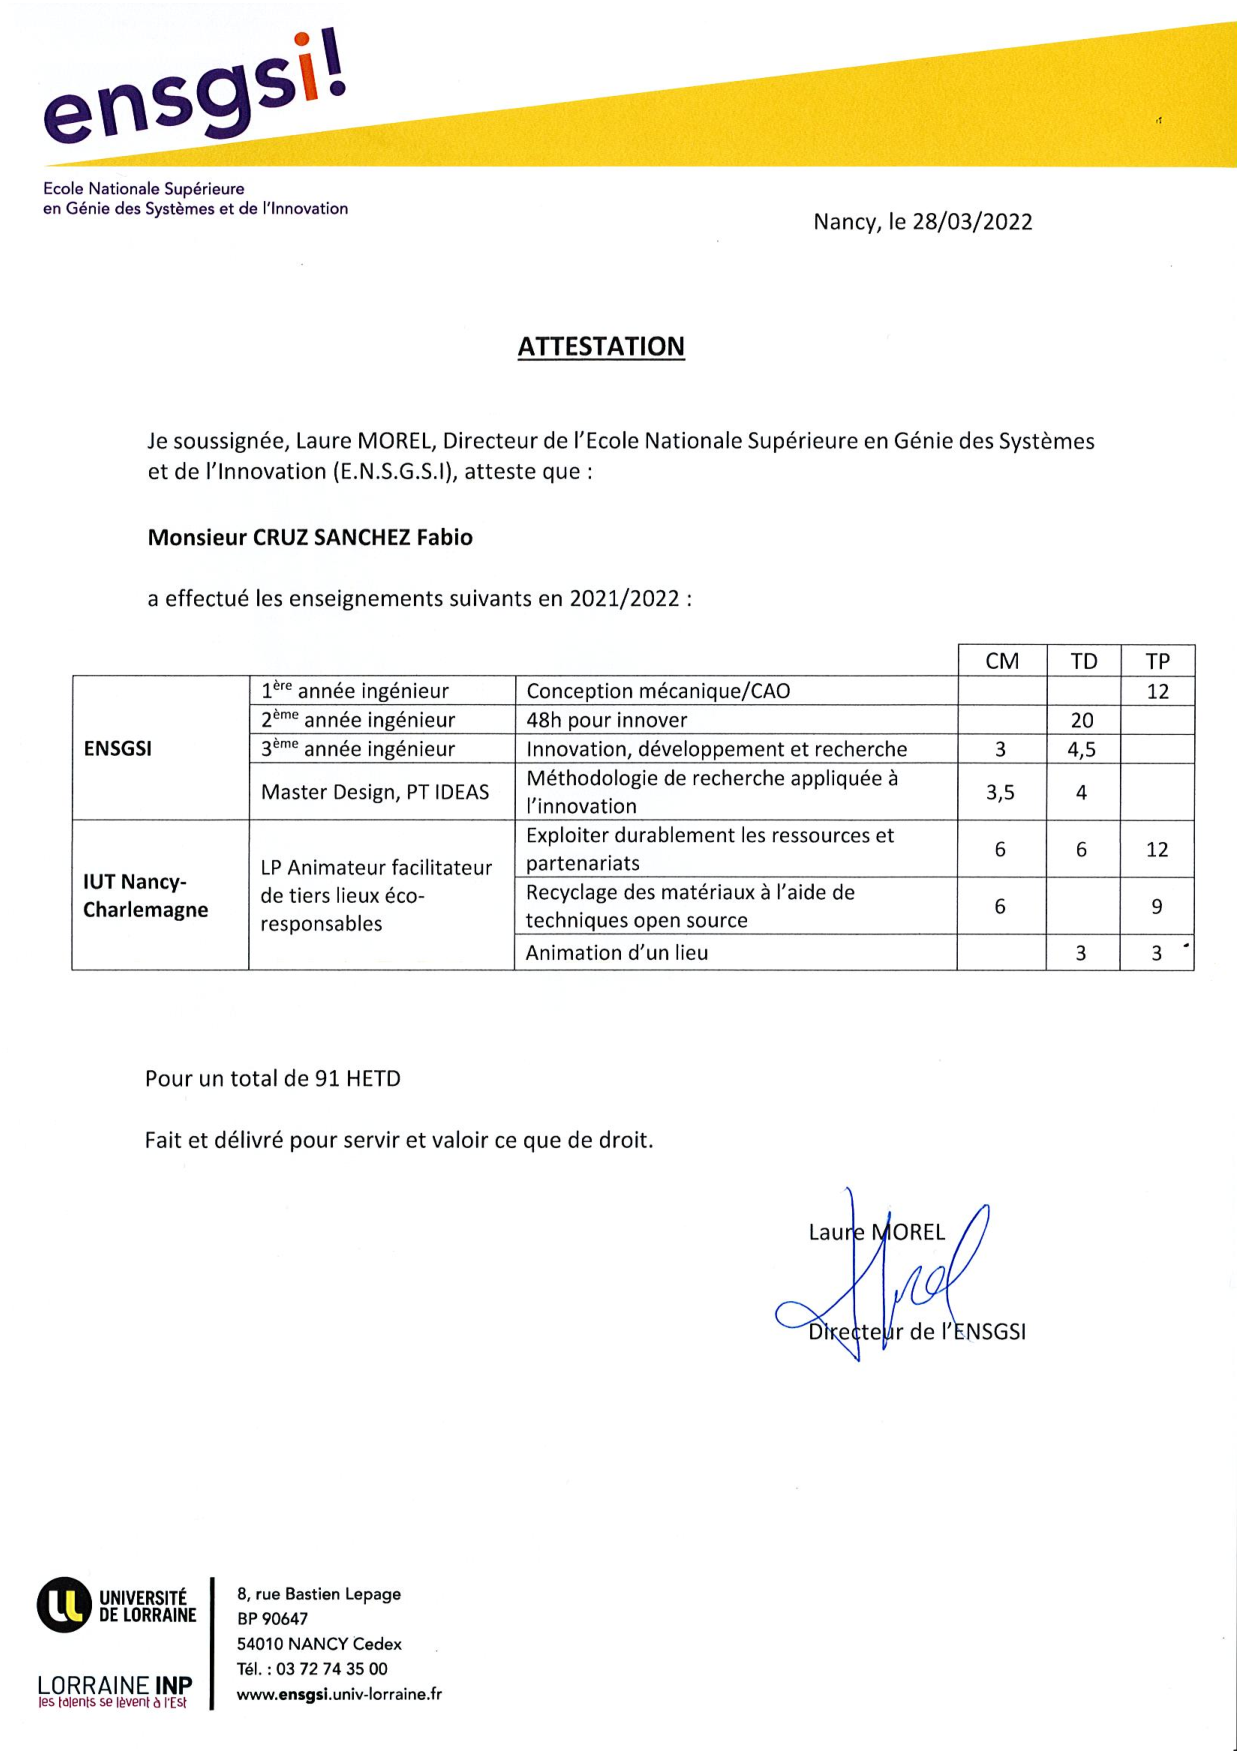
\includepdf[pages=-]{./annexs/Heures.pdf}

\end{document}
